\documentclass[12pt]{article}
\usepackage{tabularx}
\usepackage{amsmath} 
\usepackage{graphicx}
\usepackage[margin=1in]{geometry}
\usepackage{cite}
\usepackage[final]{hyperref}
\hypersetup{
	colorlinks=true,      
	linkcolor=blue,       
	citecolor=blue,       
	filecolor=magenta,    
	urlcolor=blue         
}
\usepackage{blindtext}
\usepackage{amssymb}
\usepackage{esint}
\usepackage{tikz}
\usepackage{pgfplots}
\usepackage{gensymb}
\usetikzlibrary{datavisualization}
\usetikzlibrary{datavisualization.formats.functions}
\newcommand{\Prho}{.8}%
\newcommand{\Ptheta}{55}%
\newcommand{\Pphi}{60}%
\usepackage{tikz-3dplot}
\newcommand{\uvec}[1]{\boldsymbol{\hat{\textbf{#1}}}}
%++++++++++++++++++++++++++++++++++++++++
\usepackage{empheq}

\newcommand*\widefbox[1]{\fbox{\hspace{2em}#1\hspace{2em}}}

\begin{document}

\usetikzlibrary{scopes}
\def\iangle{35} % Angle of the inclined plane

\def\down{-90}
\def\arcr{0.5cm} % Radius of the arc used to indicate angles

\title{ECE 3030 - HW 8}
\author{Joshua Tensuan - jvt24}
\date{November 7, 2022}
\maketitle


\begin{enumerate}
	\item [8.1]
	\begin{enumerate}
		\item [(a)]
		The load boundary condition tells us that,
		\[\frac{V(z=0)}{I(z=0)}=\frac{V_++V_-}{V_+/Z_0-V_-/Z_0}=Z_L\]
		Then,
		\[\Gamma_L=\frac{V_-}{V_+}=\frac{Z_L-Z_0}{Z_L+Z_0}\]
		The impedance of an inductor is given by $Z=j\omega L$.
		Since the components are connected together in series, we can find $Z_L$ by adding the individual impedances of the resistor and inductor, resulting in,
		\[Z_L = 70+j(1\cdot 10^9)(9.55\cdot 10^{-9})=70 + j9.55\]
		Substituting this in the expression for $\Gamma_L$,
		\[\Gamma_L = \frac{70 + j9.55 - 50}{70+j9.55+50}=\frac{20 + j9.55}{120+j9.55}=0.172+j0.0659\]
		\[\boxed{\Gamma_L = 0.172+j0.0659}\]

		\item [(b)]
		We know that,
		\[\begin{cases}
			V(z)=V_+\left(e^{-jkz}+\Gamma_Le^{jkz}\right) \\ 
			I(z)=\frac{V_+}{Z_0}\left(e^{-jkz}-\Gamma_Le^{jkz}\right)
		\end{cases}\]
		Thus,
		\[Z(z)=\frac{V(z)}{I(z)}=Z_0\frac{1+\Gamma_Le^{2jkz}}{1-\Gamma_Le^{2jkz}}=50\frac{1+(0.172+j0.0659)e^{2jkz}}{1-(0.172+j0.0659)e^{2jkz}}\]
		Inputting $z=-l=-21\lambda/16$, we can use the fact that $k=2\pi/\lambda$,
		\[2jkz = j\frac{4\pi}{\lambda}\cdot\frac{-21\lambda}{16}=-j\pi\frac{21}{4}\]
		Then,
		\[Z(z=-l)=50\frac{1+(0.172+j0.0659)e^{-j\pi(21/4)}}{1-(0.172+j0.0659)e^{-j\pi (21/4)}}\]
		\[Z(z=-l)=50\frac{1+(0.172+j0.0659)e^{-j\pi(5/4)}}{1-(0.172+j0.0659)e^{-j\pi (5/4)}}=35.254+j5.471\]
		\[\boxed{Z(z=-l)=\left(35.254+j5.471\right)\: \Omega}\]

		\item [(c)]
		The average power dissipated is given by $\bar P = I^2_{\mathrm{rms}}\mathrm{Re}(Z(z=-l))$.
		Letting $Z_T$ denote the total impedance in the circuit (add impedances of individual components),
		\[I_{\mathrm{rms}}=\frac{V_{\mathrm{rms}}}{|Z_T|}=\frac{5}{\sqrt{2}}\frac{1}{\sqrt{(50+35.254)^2+(5.471)^2}}\]
		\[I^2_{\mathrm{rms}}=\frac{25}{2}\frac{1}{(50+35.254)^2+(5.471)^2}=0.00171\]
		Then,
		\[\bar P = 0.00171 \cdot (35.254)=0.0604 \: \mathrm{W}\]
		\[\boxed{\bar P = 0.0604 \: \mathrm{W}}\]

		\item [(d)]
		We know that $V(z=-l)$ is equal to the voltage dissipated in $Z(z=-l)$ component in the above equivalent circuit.
		Using the phasor representation,
		\[V(z=-l)=V\cdot \frac{Z(z=-l)}{Z_s+Z(z=-l)}\]
		\[V(z=-l)=5\cdot \frac{35.254+j5.471}{50+35.254+j5.471}=2.080 + j0.187\]
		From transmission line analysis, we know that,
		\[V(z=-l)=V_+\left(e^{jkl}+\Gamma_Le^{-jkl}\right)\]
		Using the substitution of $k=2\pi/\lambda$ and $l=21\lambda/16$,
		\[kl = \frac{2\pi}{\lambda}\frac{21\lambda}{16}=\frac{21}{8}\pi\]
		Substituting this back into our expression for $V(z=-l)$,
		\[V(z=-l)=V_+\left(e^{j21\pi/8}+(0.172+j0.0659)e^{-j21\pi/8}\right)\]
		Setting our two expressions for $V(z=-l)$ equal to each other, we find that,
		\[V_+=\frac{2.080 + j0.187}{e^{j21\pi/8}+(0.172+j0.0659)e^{-j21\pi/8}}=-0.957-j2.310\]
		\[\boxed{V_+=\left(-0.957-j2.310\right)\: \mathrm{V}}\]

		\item [(e)]
		We know that $\Gamma_L=\frac{V_-}{V_+}$.
		Thus, $V_-=\Gamma_LV_+$.
		Substituting this in,
		\[V_-=(0.172+j0.0659)\cdot(-0.957-j2.310)=-0.0123-j0.460\]
		\[\boxed{V_-=\left(-0.0123-j0.460\right)\: \mathrm{V}}\]

		\item [(f)]
		We know that the time-averaged power in the $+z$-direction is given by (derivation given in lecture),
		\[\langle P_z(t)\rangle = \frac{1}{2}\mathrm{Re}\left[\frac{|V_+|^2}{Z_0^*}-\frac{|V_-|^2}{Z_0^*}\right]\]
		Substituting this in via Mathematica, we find that,
		\[\langle P_z(t)\rangle = 0.0604\:\mathrm{W}\]
		\[\boxed{\langle P_z(t)\rangle = 0.0604\:\mathrm{W}}\]
		We notice that this is identically equal to our answer from part c.
		Thus, the net time-average power traveling in the $+z$-direction in the transmission line circuit is equal to the time-averaged power dissipated by the equivalent impedance component $Z(z=-l)$.

		\item [(g)]
		To find $Z_{\mathrm{th}}$, we can short the voltage source and find the impedance looking in from both terminals, resulting in,
		\[\Gamma_s=\frac{V_+}{V_-}=\frac{Z_s-Z_0}{Z_s+Z_0}\]
		\[\Gamma_s=\frac{50-50}{50+50}=0\]
		Then,
		\[Z_{\mathrm{th}}=Z_0\frac{1+\Gamma_se^{-2jkl}}{1-\Gamma_se^{-2jkl}}=50\]
		To find $V_{\mathrm{th}}$ we remove the load (break the circuit) and find the voltage at the terminals.
		\[V_{\mathrm{th}}=2V_+=\frac{V_s}{\cos(kl)}\cdot\frac{-jZ_0\cot(kl)}{Z_s-jZ_0\cot(kl)}\]
		Using the fact that $kl=21\pi/8$,
		\[V_{\mathrm{th}}=\frac{5}{\cos(21\pi/8)}\cdot \frac{-j50\cot(21\pi/8)}{50-j50\cot(21\pi/8)}=-1.913-j4.619\]
		\[\boxed{\begin{cases}
			Z_{\mathrm{th}} = 50 \: \Omega \\ 
			V_{\mathrm{th}} = (-1.913-j4.619) \: \mathrm{V}
		\end{cases}}\]

		\item [(h)]
		The average power dissipated is given bt $\bar P = I_{\mathrm{rms}}^2\cdot R$.
		Letting $Z_T$ denote the total impedance in the circuit (add impedances of individual components),
		\[Z_T = Z_{\mathrm{th}}+R+j\omega L = 50+70 + j(1\cdot 10^9)(9.55\cdot 10^{-9})=120+j9.55\]
		Then,
		\[I_{\mathrm{rms}}=\frac{V_{\mathrm{rms}}}{|Z_T|}=\frac{|-1.913-j4.619|}{\sqrt{2}}\cdot\frac{1}{\sqrt{120^2 + 9.55^2}}\]
		\[I_{\mathrm{rms}}^2 = \frac{1.913^2+4.619^2}{2}\cdot\frac{1}{120^2+9.55^2}=0.000863\]
		Then,
		\[\bar P = I^2_{\mathrm{rms}}\cdot 70 = 0.0604 \: \mathrm{W}\]
		\[\boxed{\bar P = 0.0604 \: \mathrm {W}}\]
		We notice that this is once again identical to our answer from part c and part f.
		Thus, the net time-average power traveling in the $+z$-direction in the transmission line circuit is equal to the time-averaged power dissipated by the equivalent impedance component $Z(z=-l)$ is equal to the time-averaged power dissipated by the load resistor in the Thevenin-equivalent circuit.
		In other, less terse words, this tells us that the load resistor dissipates a 100\% of the power that is dissipated by the transmission line and load 'part' of the circuit.
		Thus, no true power is dissipated in the transmission line and instead all the true power is dissipated in the load resistor.

	\end{enumerate}

	\item [8.2]
	\begin{enumerate}
		\item [(a)]
		We know that $Y_0=1/Z_0$.
		Then, $Y(z)=1/Z(z)$ and $Y_n(z)=Y(z)/Y_0=1/Z_n(z)$.
		\[Y_n(z=0)=\frac{1}{Z_n(z=0)}=2\]
		Using the Smith chart to find $l_1$ as shown below,
		
		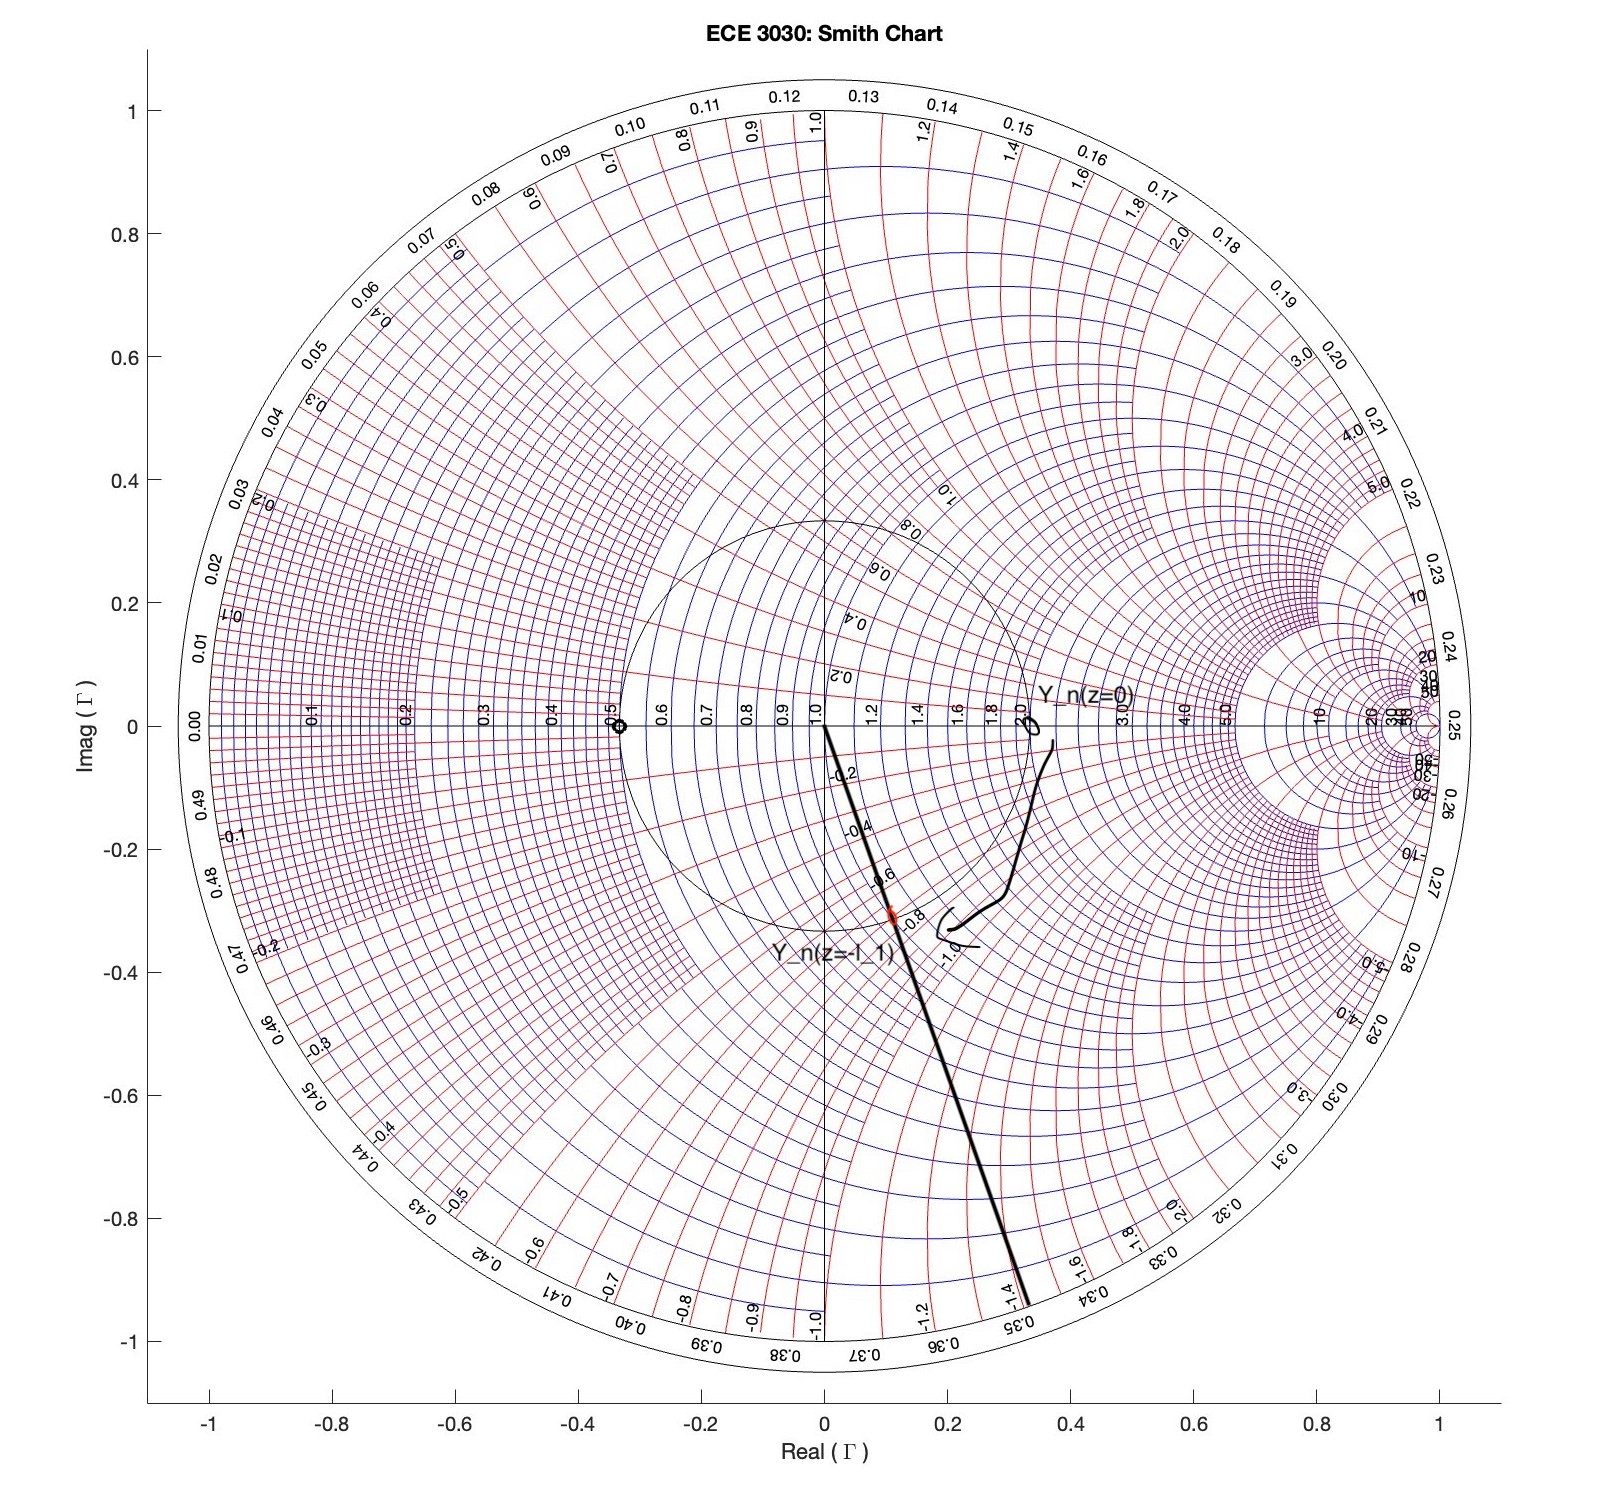
\includegraphics[width = 5in]{images/ece3030-q2-1.jpg}

		We find that $l_1\approx 0.348-0.25 = 0.098$.
		Thus,
		\[\boxed{l_1=0.098\lambda}\]

		\item [(b)]
		For an open circuit stub tuner, we treat $Z_n(z=0)=\infty$ and $Y_n(z=0)=0$.
		From the previous part, we find that the imaginary part of the admittance is roughly $-0.7j$.
		Thus, in order to cancel out this imaginary part of the admittance, we want our open-circuit parallel stub tuner to have an imaginary part of admittance be $+0.7j$.
		Using the Smith chart to find $l_2$ as shown below,

		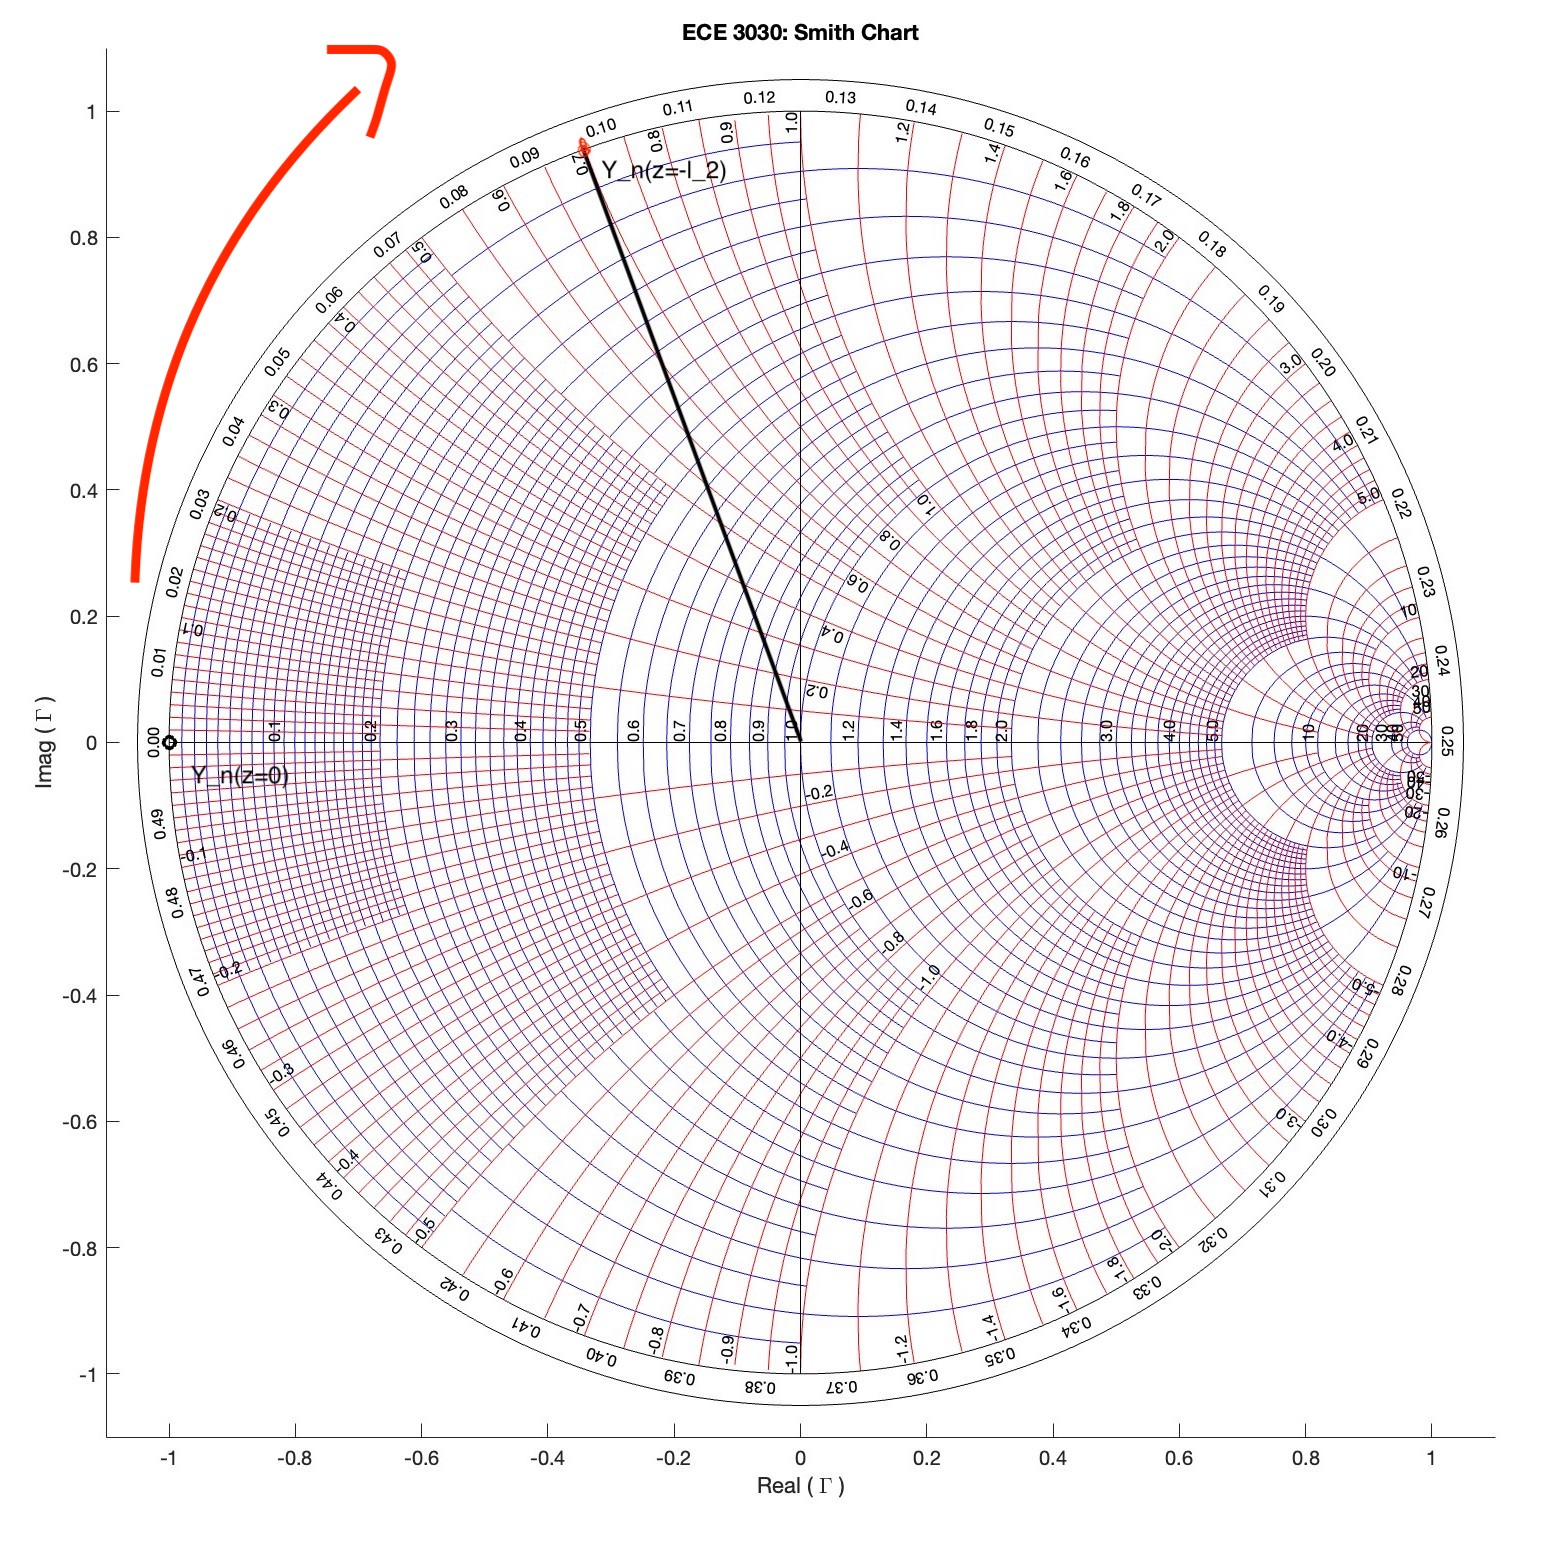
\includegraphics[width = 5in]{images/ece3030-q2-2.jpg}

		We find that $l_2 \approx 0.097$.
		Thus,
		\[\boxed{l_2=0.097 \: \lambda}\]


	\end{enumerate}

	\item [8.3]
	We begin by finding the necessary length of the transmission line, $l_1$, to 'cancel' out the resistance of the load.
	We want to find the desired $l_1$ such that $Z_n(z=-l_1)=1.0+jX_n$.
	We know that $Z_n(z=0)=Z_L/Z_0=0.6-j0.8$.
	Using the Smith chart as found below, we find that,

	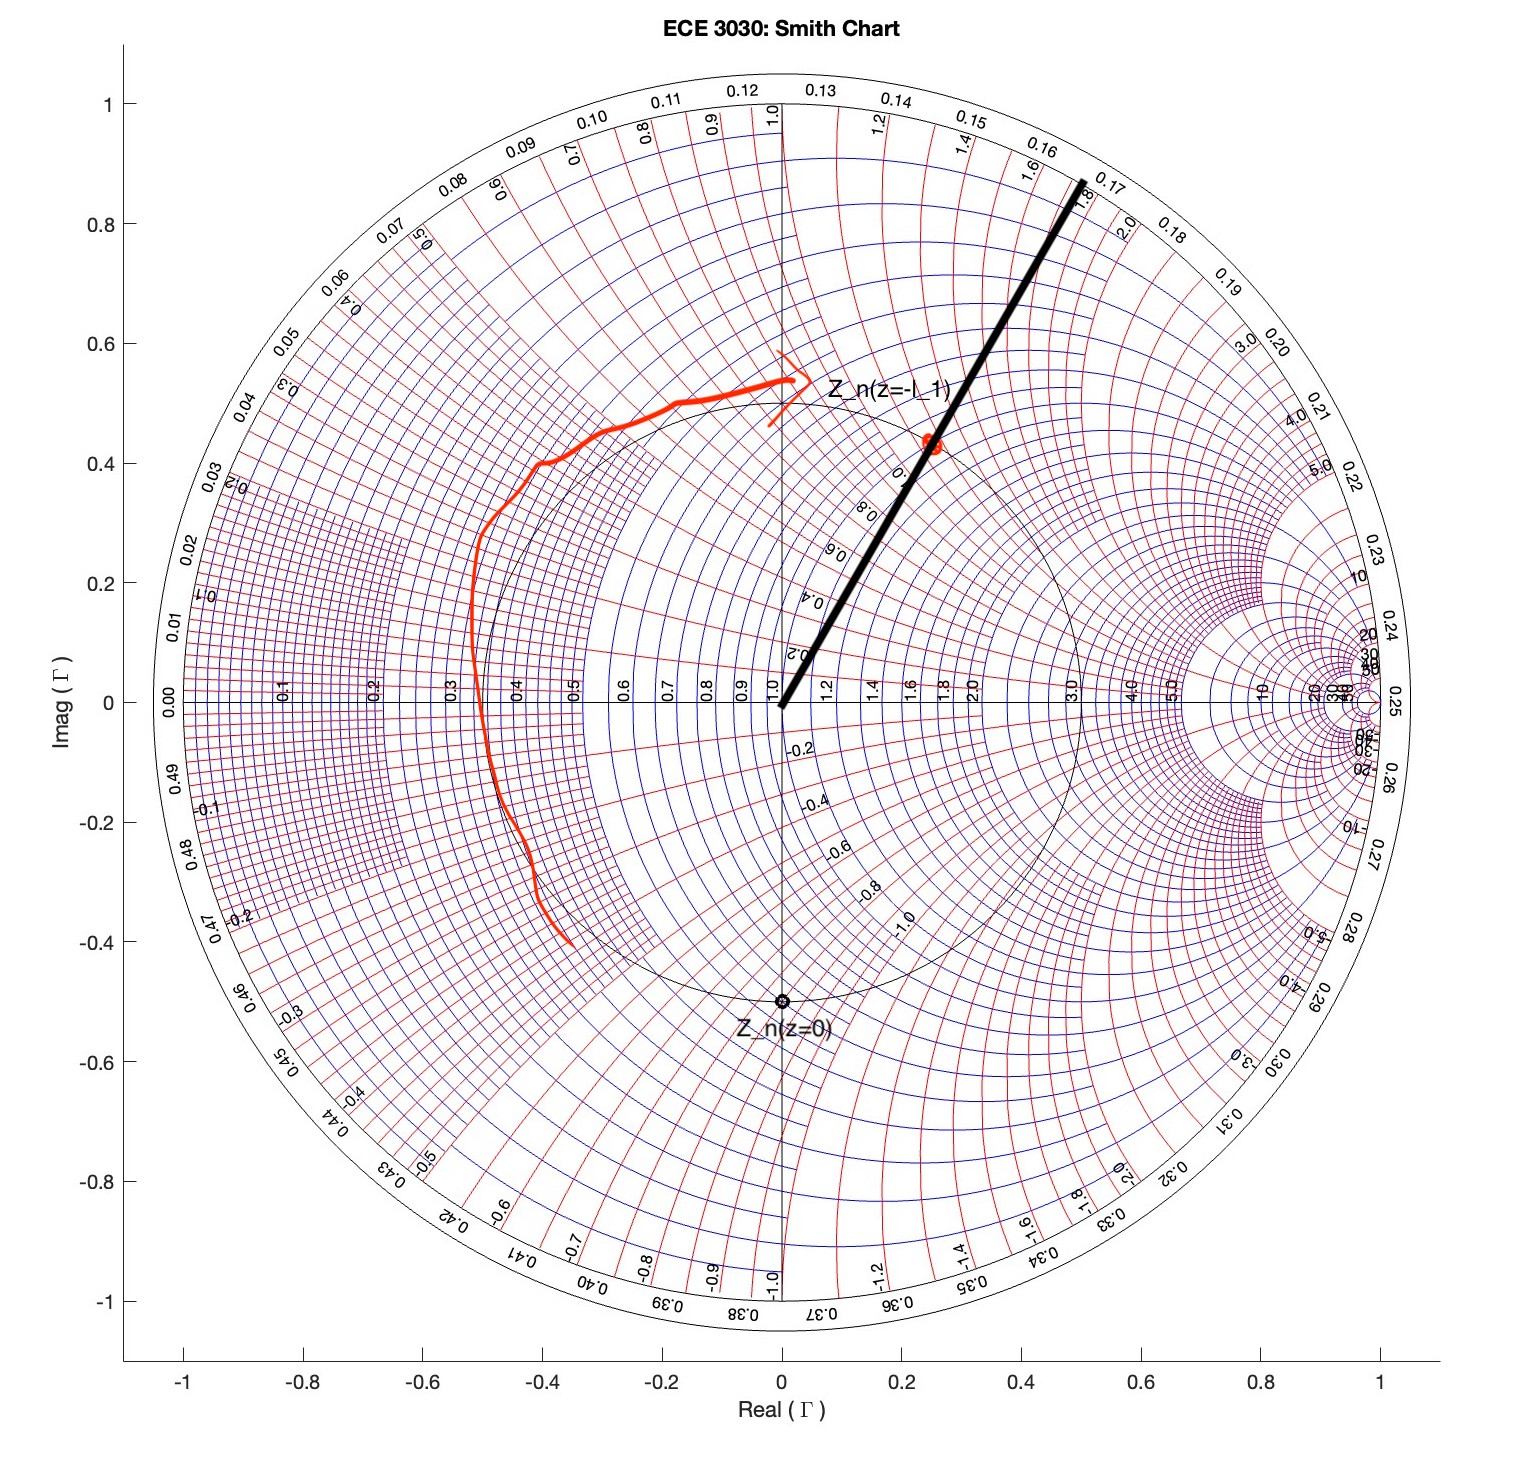
\includegraphics[width=5in]{images/ece3030-q3-1.jpg}

	$l_1\approx 0.5+0.167-3/8=0.292\lambda$.

	This gives us,

	\[Z_n(z=-l_1)=1.0 + j1.15\]

	Thus, the actual impedance $Z(z=-l_1)=Z_n(z=-l_1)\cdot Z_0 = (100 + j115)\:\Omega$.

	Let us begin by analyzing a stub tuner in series.
	Thus, we want $Z(z=-l_2)=-j115 \: \Omega \to Z_n(z=-l_2)=-j1.15$ to cancel out the unwanted reactance.

	Since negative reactances are on the bottom right of the Smith chart, we want to start on the right side of the Smith chart (corresponds to an open-circuit stub tuner).
	Finding $l_2$ using this Smith chart, we find that with the series setup,

	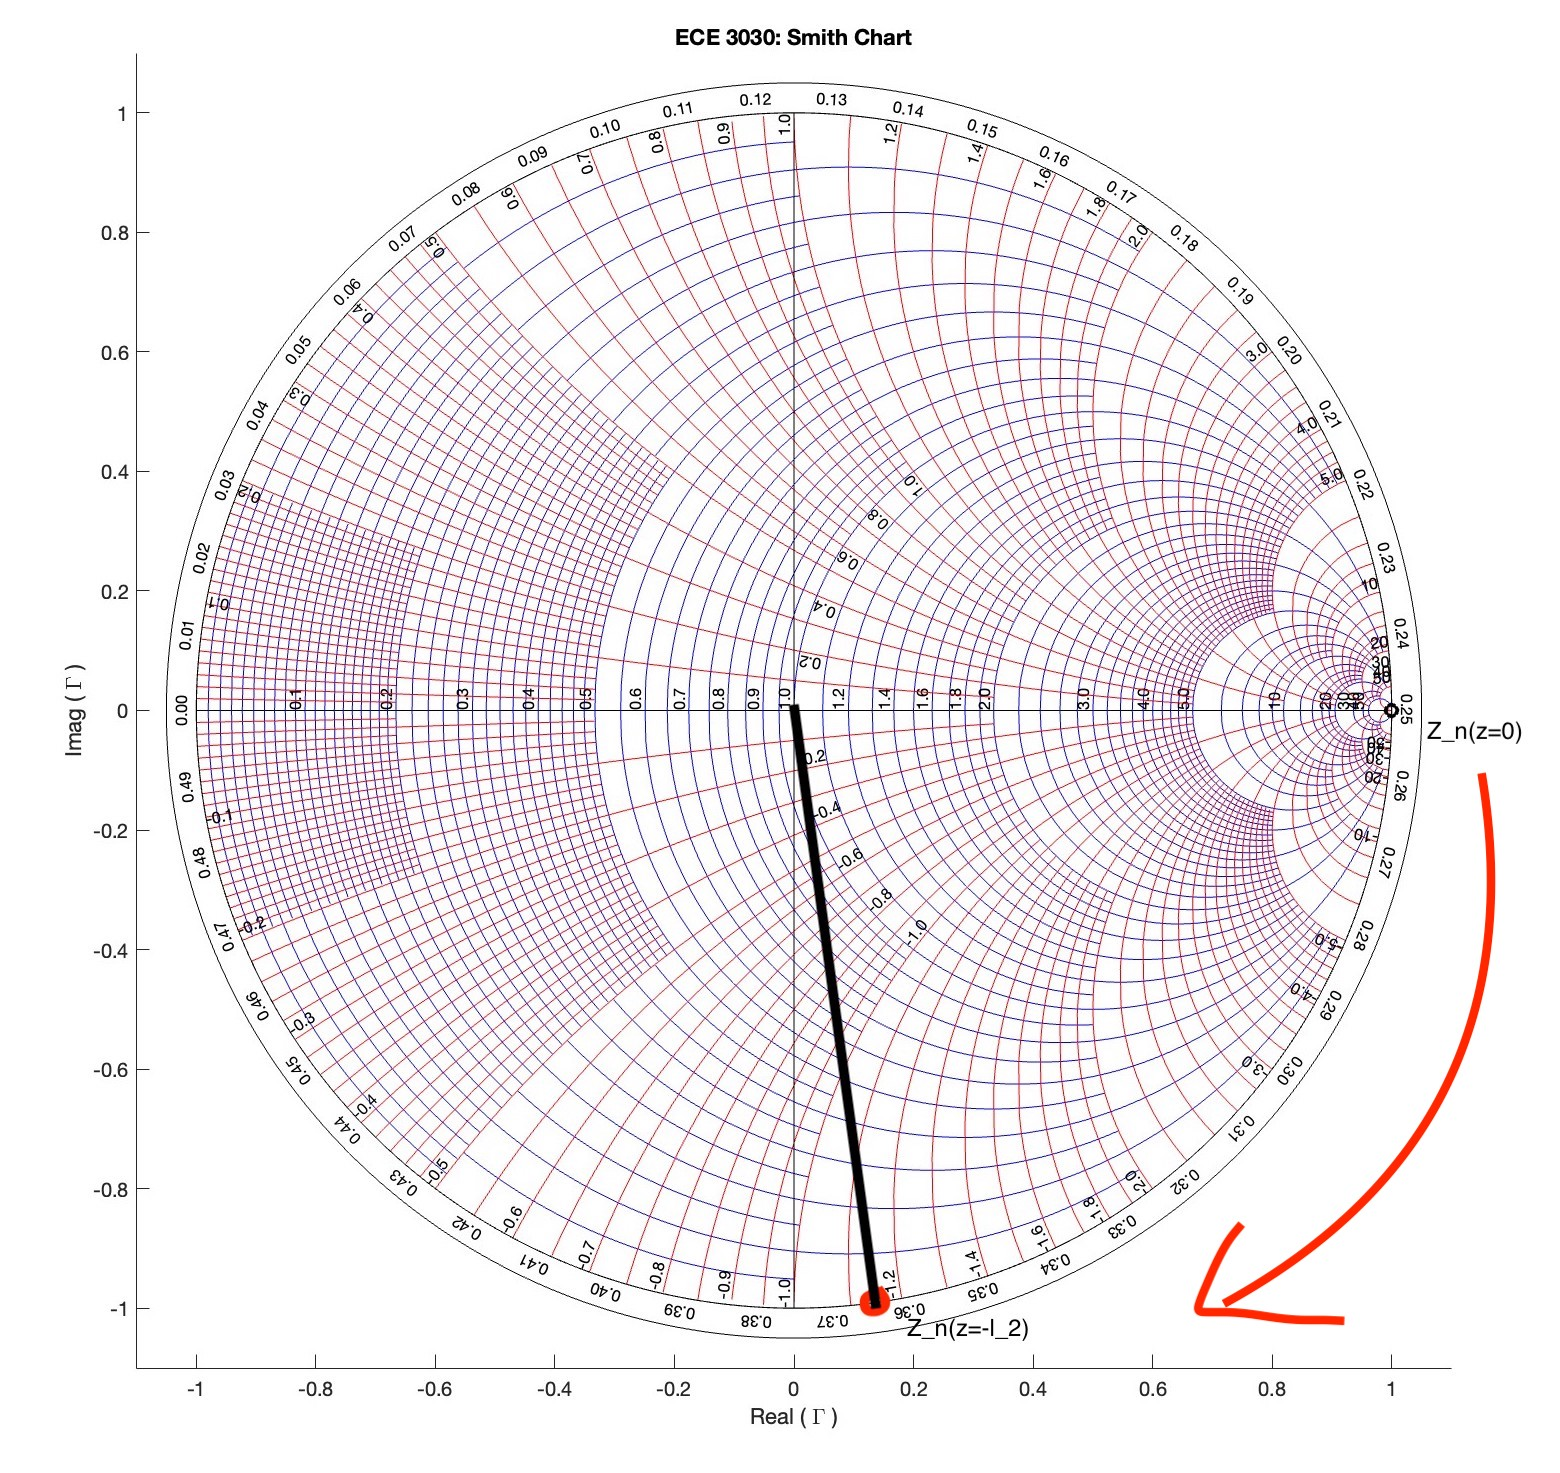
\includegraphics[width = 5in]{images/ece3030-q3-2.jpg}

	$l_2\approx 0.364-0.25=0.114\lambda$.
	Thus, for a stub tuner in series, we have a total length of $0.406\lambda$.

	Let us now analyze the stub tuner in parallel.
	We have admittance $Y_n(z=0)$ of,
	\[Y_n(z=0)=\frac{1}{Z_n(z=0)}=0.6+j0.8\]
	We want to find the desired $l_1$ such that $Y_n(z=-l_1)$ has a real part equal to unity.
	Using the Smith chart below, we find that,

	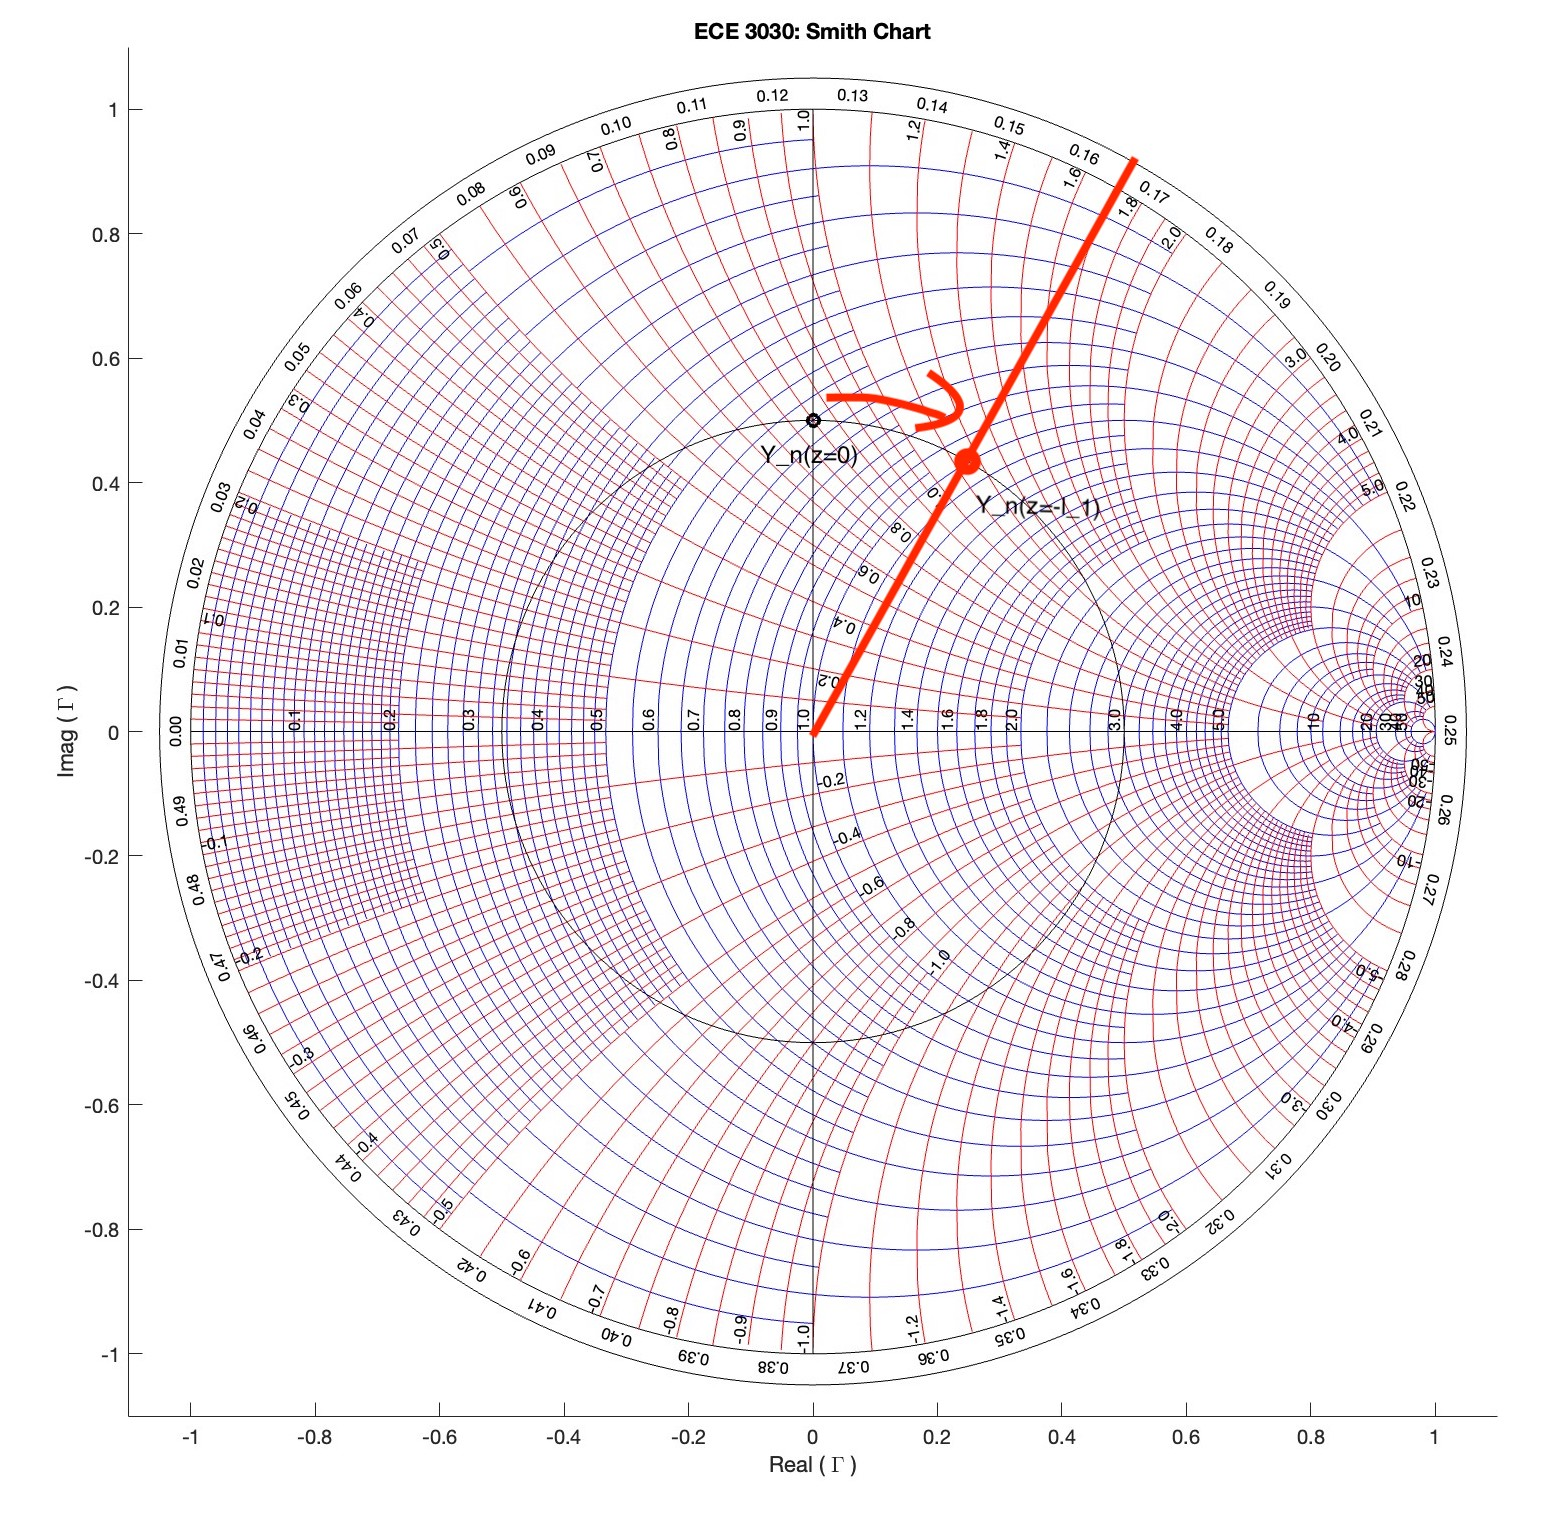
\includegraphics[width=5in]{images/ece3030-q3-3.jpg}

	$l_1\approx 0.166-1/8=0.041\lambda$.

	This gives us,
	\[Y_n(z=-l_1)=1+j1.15\]

	Thus, we want $Y(z=-l_2)=-j1.15$ to cancel out the unwanted imaginary part of the admittance.

	If we want a negative imaginary part of the admittance, we want to start on the right side of the Smith chart (corresponds to a closed-circuit stub tuner in parallel).
	Finding $l_2$ using this Smith chart, we find that with the parallel setup,

	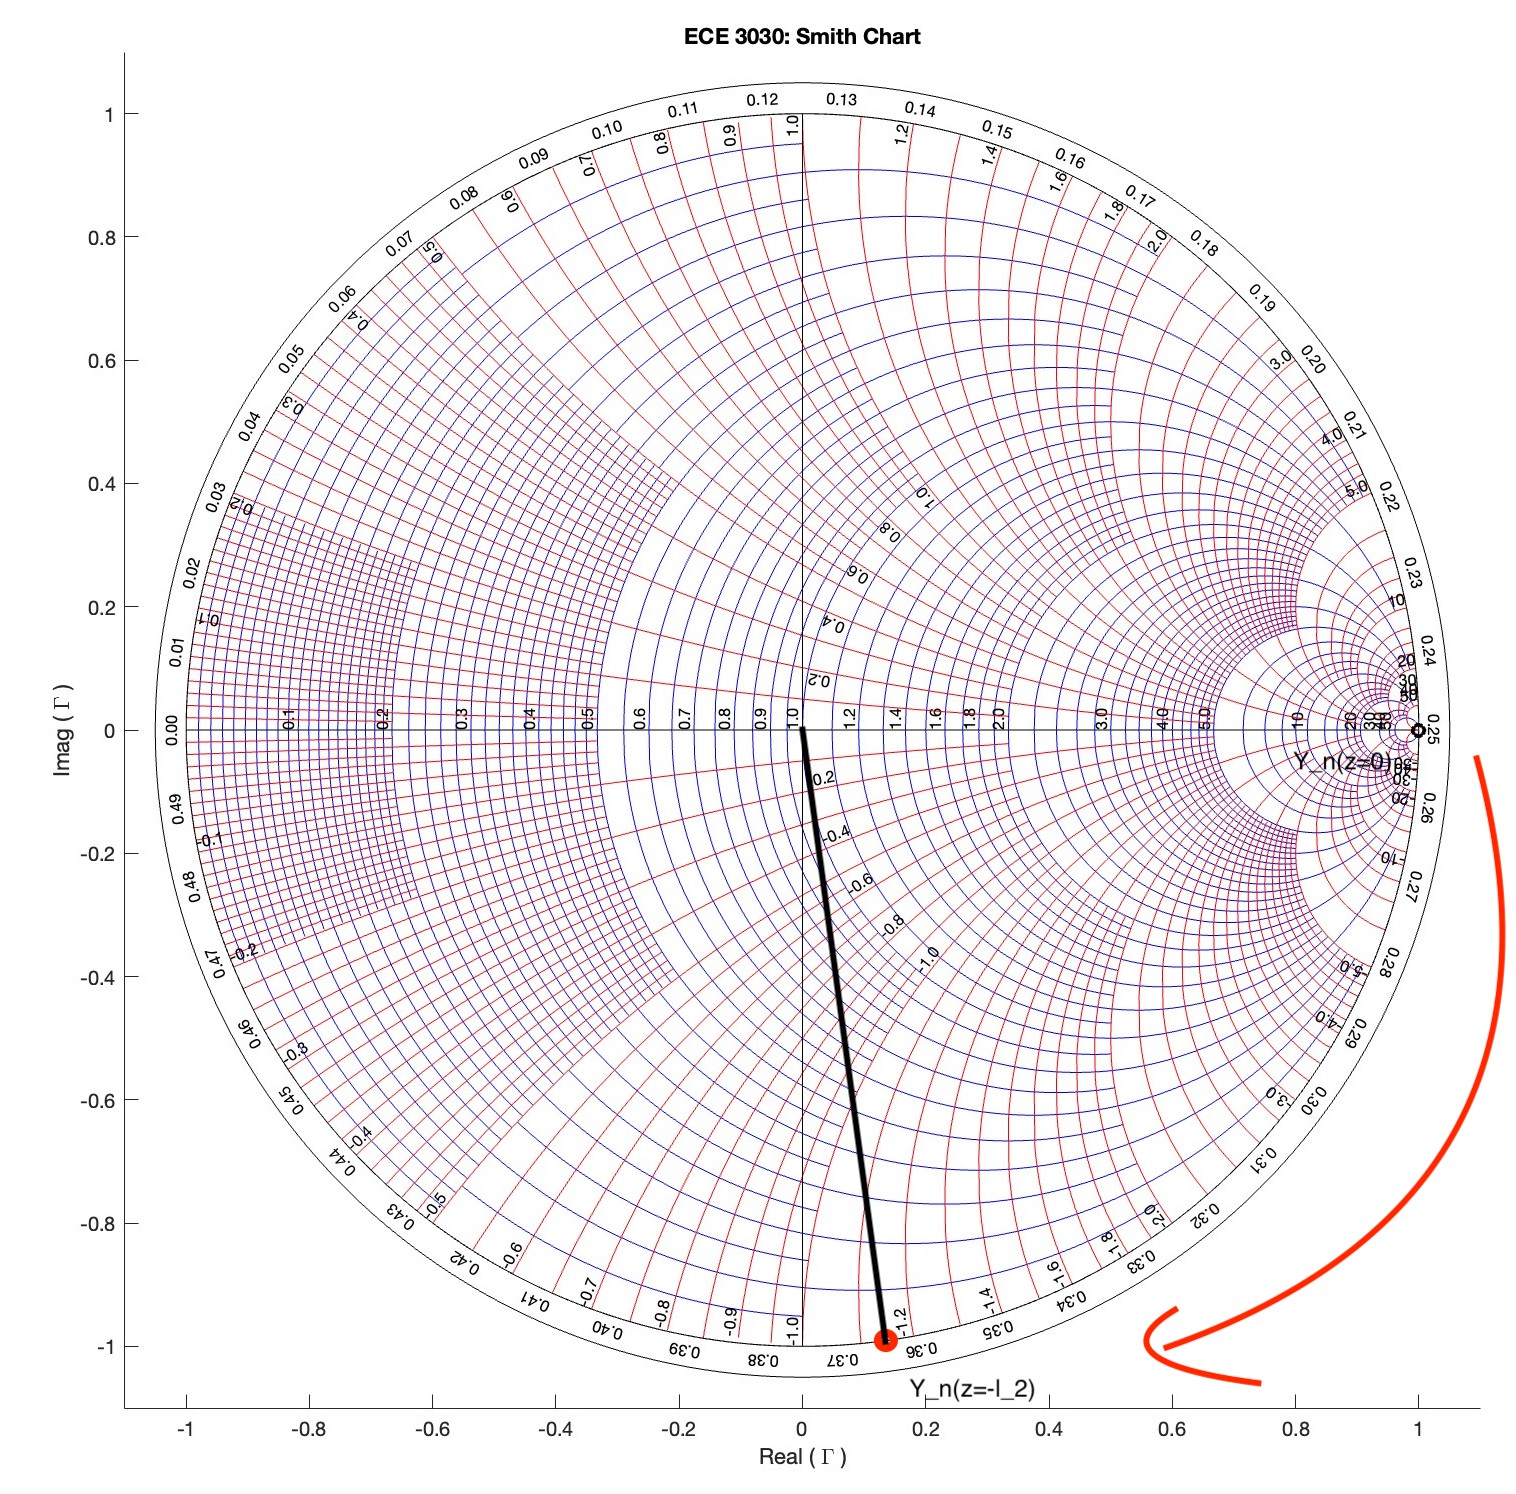
\includegraphics[width=5in]{images/ece3030-q3-4.jpg}

	$l_2\approx 0.364-0.25 = 0.114 \lambda$.

	Thus, for a stub tuner in parallel, we have a total length of $0.141 \lambda$.

	Thereby, to place the stub as close as possible and have a stub that is as short as possible, we have a short-circuit stub tuner in parallel of length $0.114 \lambda$ place $0.041\lambda$ from the load.
	In other words, we have a transmission line of length $0.041 \lambda$ between the load and the stub.

	\[\boxed{\text{Short-circuit stub tuner in parallel.}}\]







		
\end{enumerate}

		

\end{document}
